\section{Time box 1}
\subsection{Time box planning}
Overview of the what work is put into which time boxes.
\begin{figure}[H]
	\begin{centering}
		 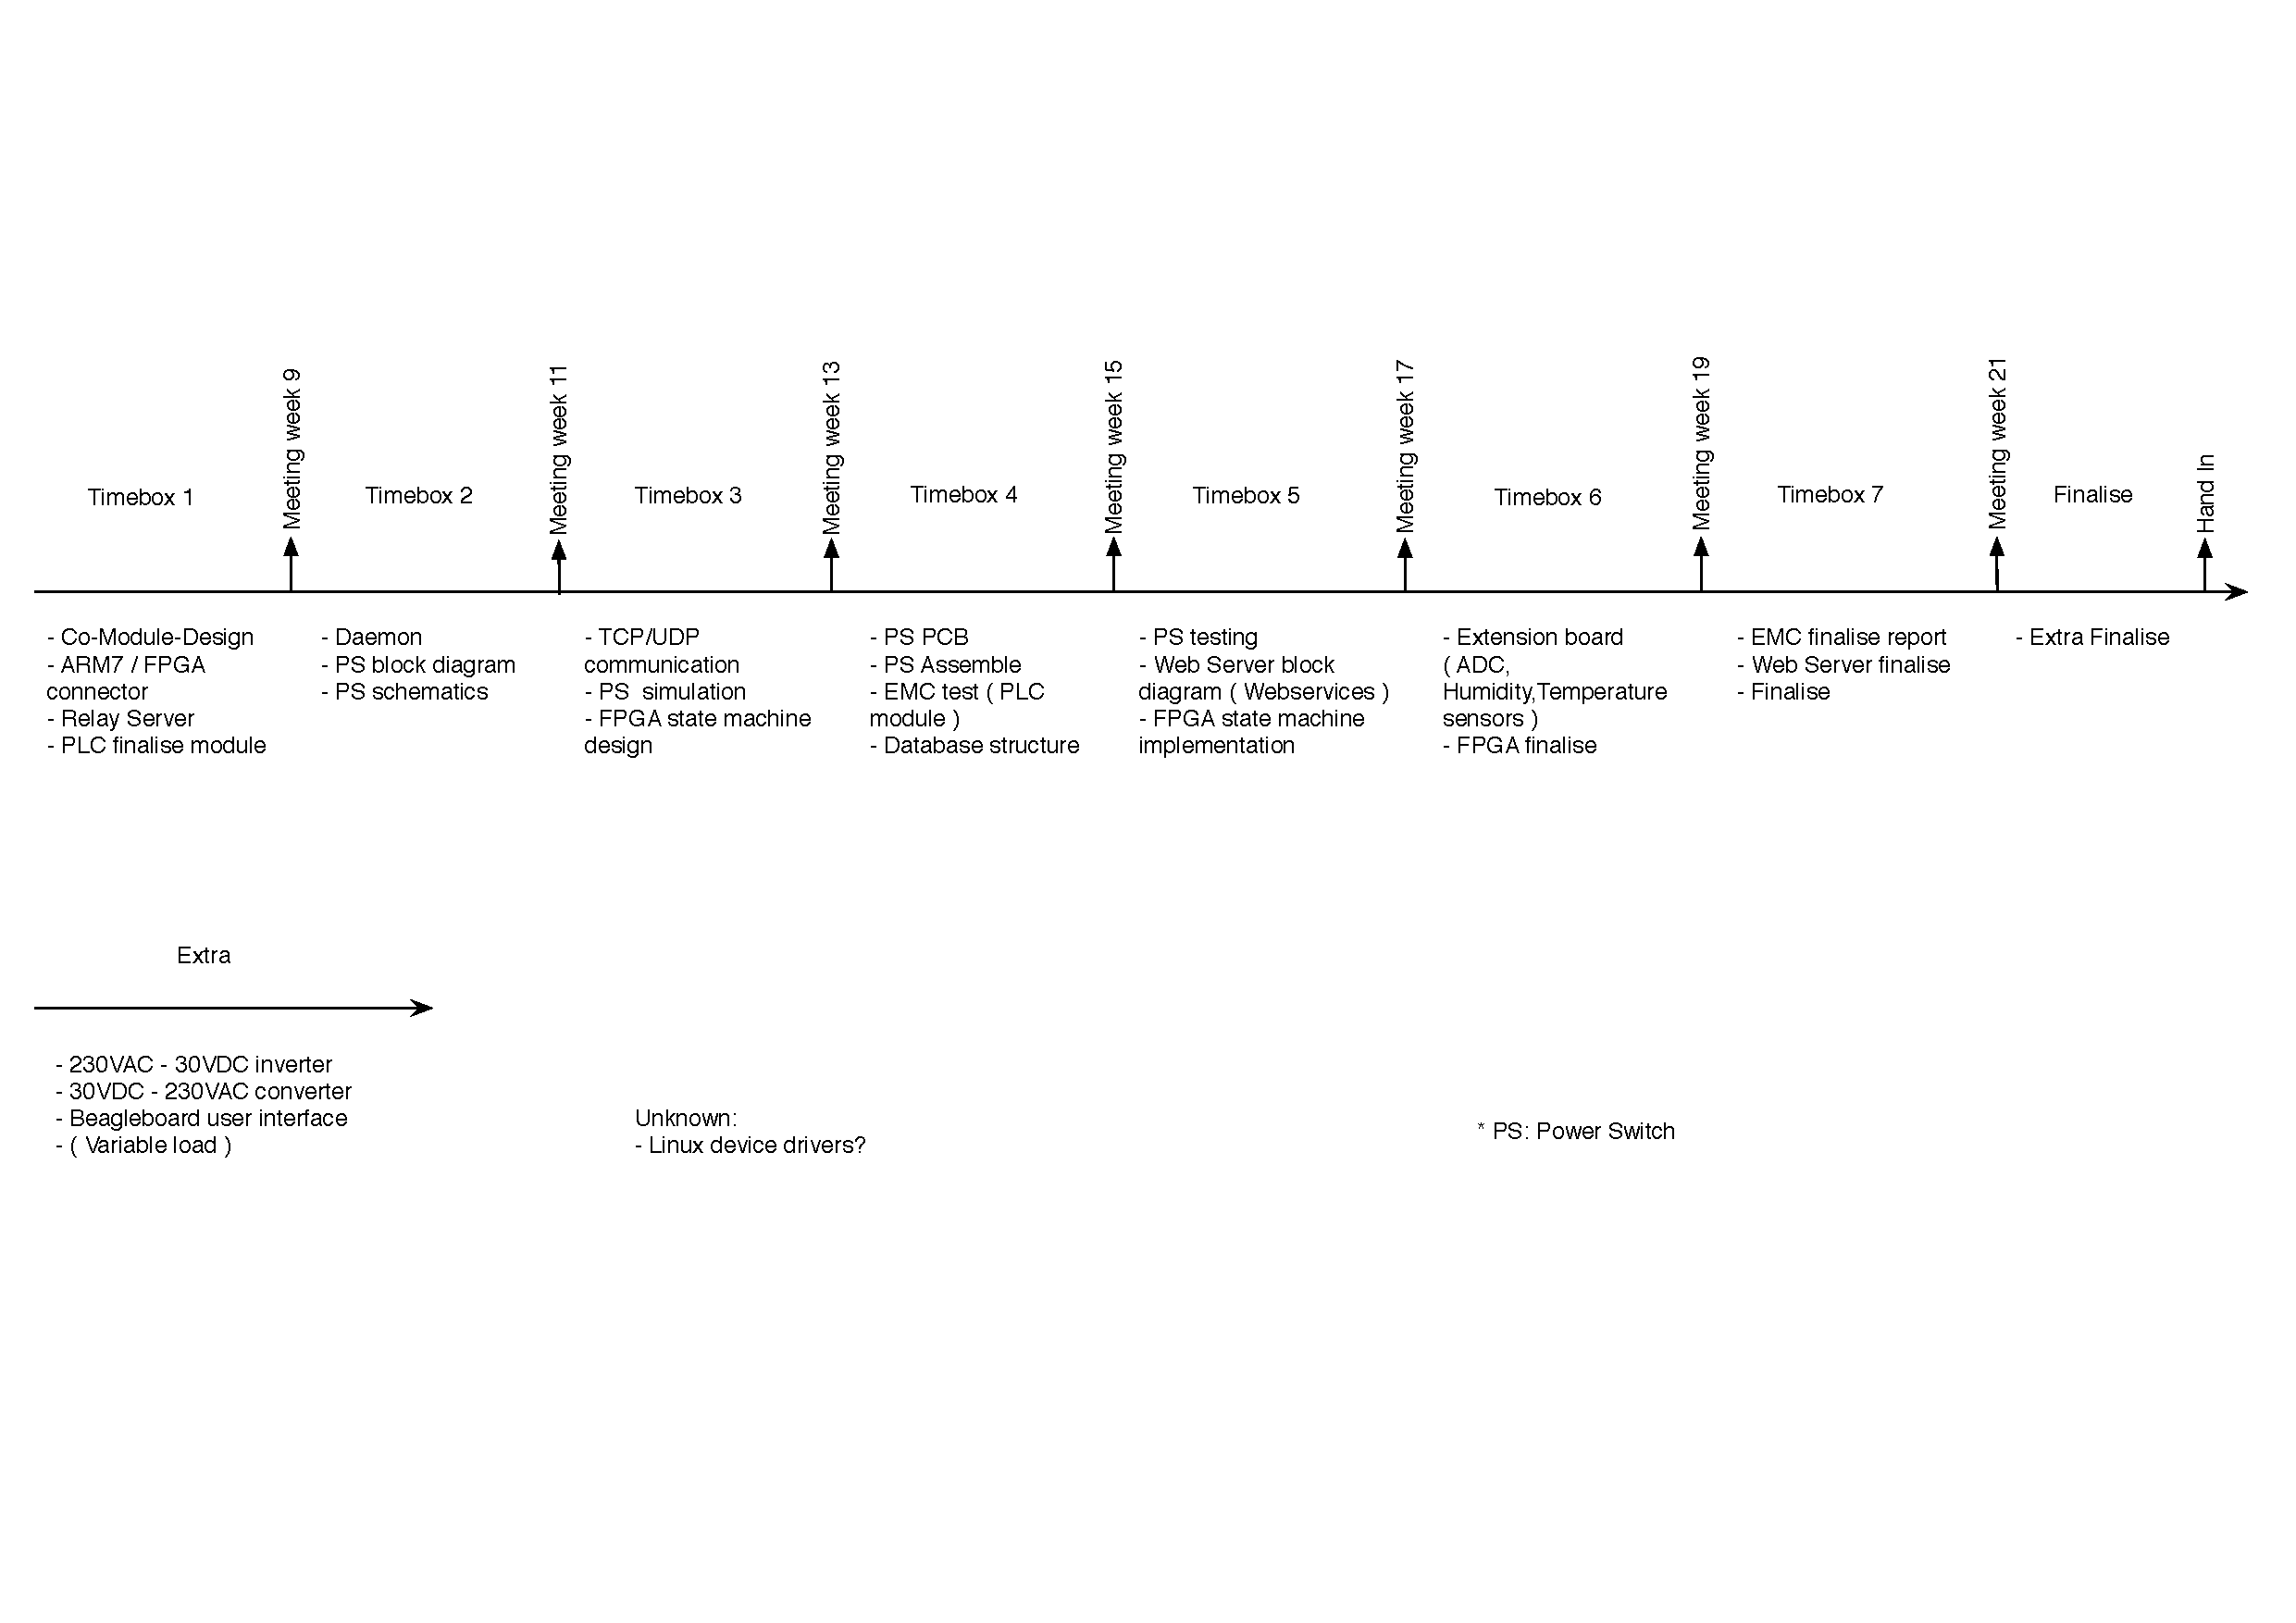
\includegraphics[width=1.0\textwidth]{content/appendix/eudp/images/tb_r1.pdf}
		\caption{Outline of the time-boxes}
	\end{centering}
\end{figure}

\subsubsection{Work to be done in this time box}
\begin{itemize}
	\item CO-Module-design
	\item Print connector (connector board between the FPGA board and the ARM board used).
	\item Relay server
	\item PLC module (Power line module for communication between the modules)
\end{itemize}

\subsection{Interface analysis (ARM to FPGA) - Dennis}
Interfacing the FPGA board (in our case a Spartan6 board by Digilent and the Arm board from EA) can be done in different ways. The fastest way if the number of connections are relatively low, is usually with a bunch of wires between the two boards. But even though such a set-up can be much more flexible, it can be very hard to error searching if something is not working (because of a broken wire or a short circuit) and is also very sensitive to noise. Instead of the wires a PCB solution has been chosen, which will be designed to fit between the two boards pin headers. By placing the boards next to each other an approximation of the board size is found. Size of the board is set to 16 x 5 cm. The connections available on the FPGA boards extension pins is 28, so a 32 bit connection is not a possibility, instead a 16 bit data connection is chosen. The pins routed between the ARM and the FPGA is:
\begin{itemize}
	\item 16 x Data
	\item 7 x Address
	\item 1 x Chip select
	\item 1 x Write enable 
	\item 1 x Output enable (read enable)
	\item 1 x interrupt to the ARM processor
	\item 1 x Reset from the ARM board
\end{itemize}
The reset pin is used for synchronous reset of the two boards. The interrupt signal makes it possible for the FPGA to interrupt the ARM board. The chip select is used, as two other devices is also connected to the external memory.
\begin{figure}[H]
	\begin{centering}
		 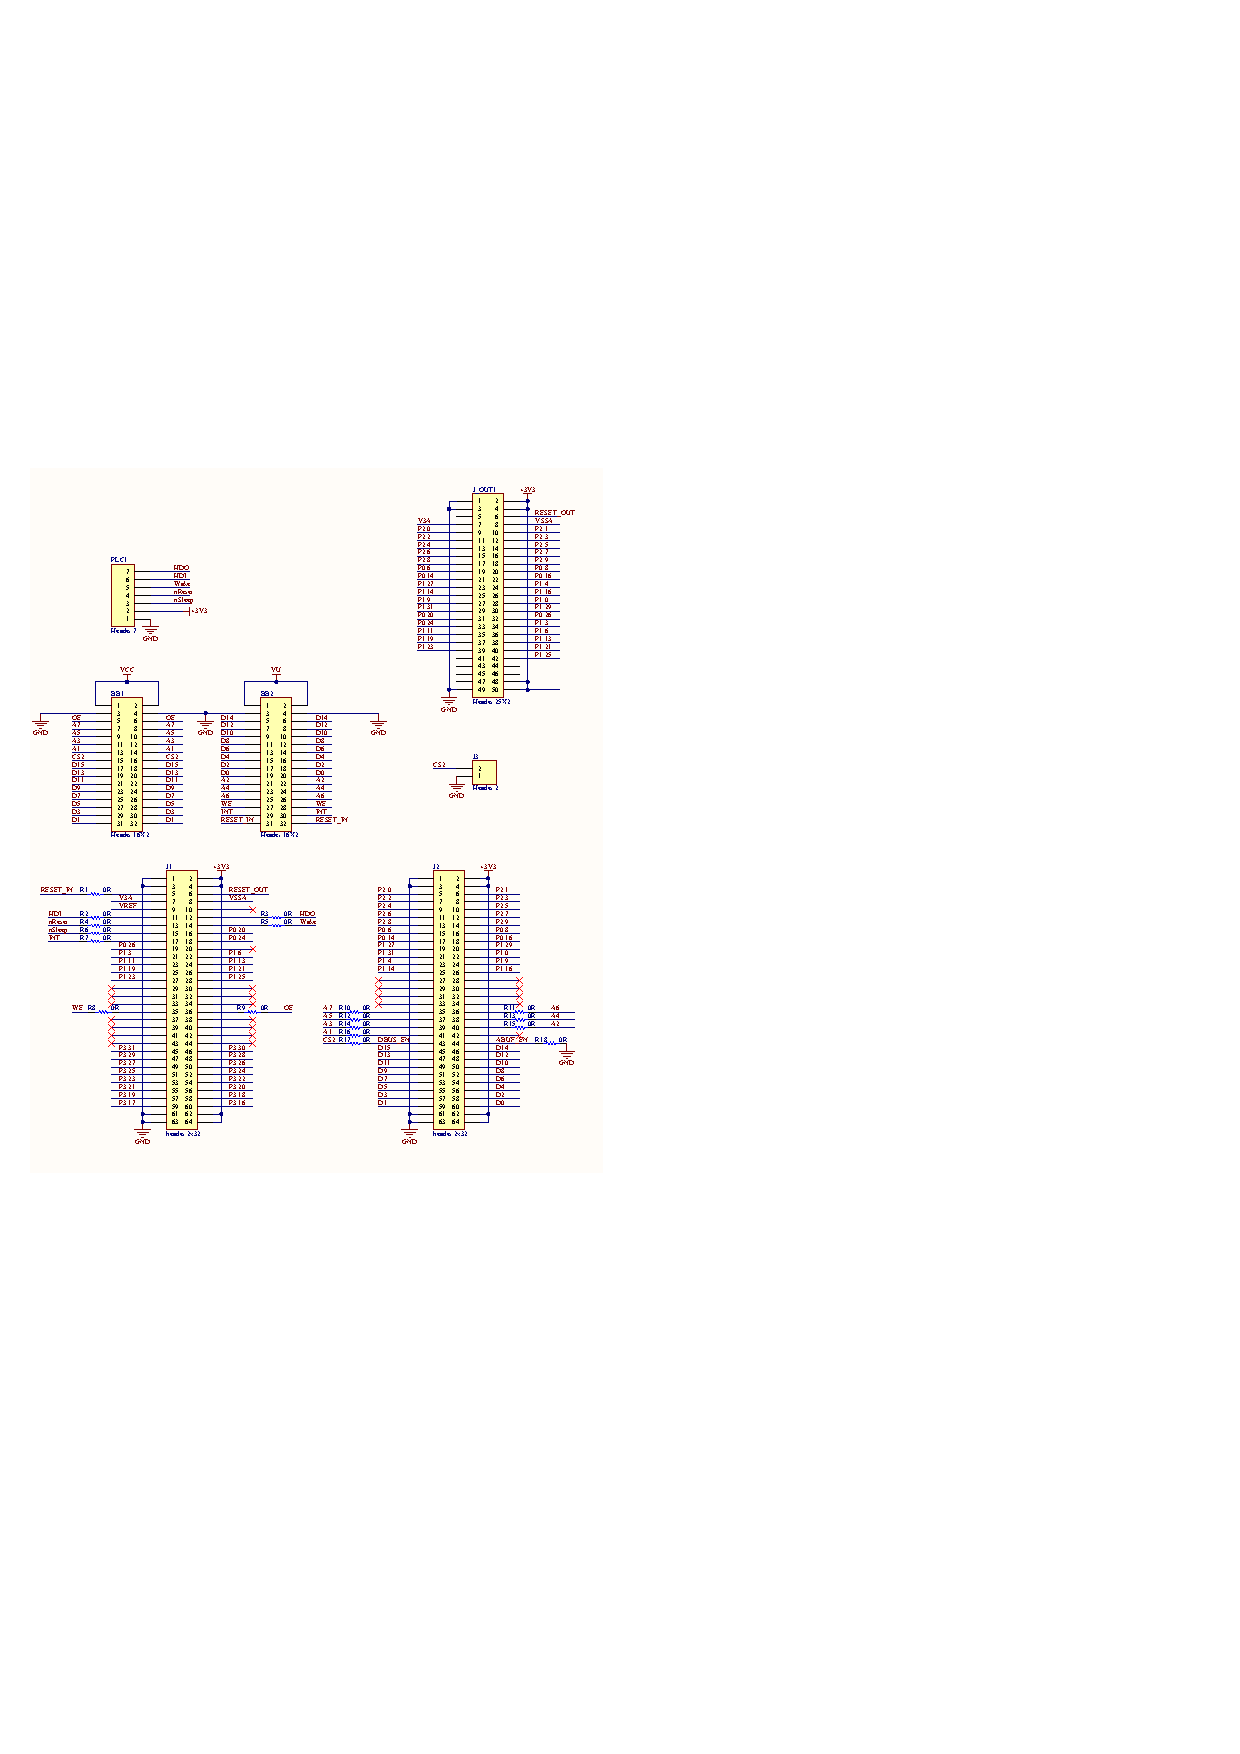
\includegraphics[width=0.60\textwidth,page=1]{content/appendix/eudp/images/dig_to_ea_v0_1}
		\caption{Schematic of the ARM to FPGA connector.}
	\end{centering}
\end{figure}
A connector for the power line module is also mounted, to easily interface the module with the ARM processor. An pin header with all the unused pins is also added, to make it possible to quickly connect external devices to the processor. 
\begin{figure}[H]
	\begin{centering}
		 \includegraphics[height=0.8\textwidth,page=2,angle=90]{content/appendix/eudp/images/dig_to_ea_v0_1}
		\caption{PCB of the ARM to FPGA connector (top view)}
	\end{centering}
\end{figure}

\subsection{Concurrent design - Theis}
Concurrent design in the design of embedded system is a method to decided where to place different parts of the system, from the specification and performance requirements. The difference between traditional design and co-design is, in traditional design, two groups of experts design independently hardware and software, to implement when all is finish. In co-design one group is designing the whole system and implement the part where they get the best performance and power use.\\
Concurrent design has four steps that is:
\begin{enumerate}
	\item Modelling
	\item Partitioning
	\item Concurrent synthesis
	\item Concurrent simulation
\end{enumerate}
In this time box, only the two first steps are described according to the project time plan.

\subsubsection{Modelling}
In the modelling phase, the customers needs is taking into consideration, and the platform for the system is choose. In this project the platform is specified from the project requirements, to include an ARM7 CPU with uClinux as processor in the system, and a Spartan 6 or 3 FPGA for hardware parts in the system.

\subsubsection{Partitioning}
In "technical platform" from the launch phase, the hardware and software specification was made, and the table below shows which parts of the project that can be implemented both in the ARM7 CPU as software and in the FPGA as hardware.

\begin{itemize}
	\item PLC module
	\item Power switch
	\item A/D Converter
	\item Ethernet
	\item Web server
	\item Interface
	\item Indicator
\end{itemize}
\textbf{PLC module} is used to communicate with the other modules, this part is best implemented in the ARM7 CPU as software, because it is a data-communication protocols.\\
\textbf{Power switch} is used to control the switch and is a rather complex algorithm, it have to be dynamic when controlling the switch, because the power consumption and production is never the same, this part is best implemented in software for the ARM7 CPU.\\
\textbf{A/D Converter} is a very suitable part to implement in the FPGA as hardware, the frequency is high, the memory requirement is small, the task is static. And in this project there is more than one A/D converter, so it is good to run this part in parallel.\\
\textbf{Ethernet} is made in software, and supported by the linux kernel. The embedded arm board have a dedicated IC (PHY) to handle communication between ethernet and the CPU\\
\textbf{Interface/Indicator} is the buttons and LEDs where the user can interact with the system, this is put into hardware, because it is IOs that is best handle in the FPGA for parallel reading the inputs and setting outputs.

\subsection{Relay-server - Paulo}
Relay server is programmed in C++, this application will run on the development platform so remote access to the EA-LPC2478 board becomes possible.

\begin{itemize}
	\item Requirements
	\item Setting the scene
	\item Server data flow
	\item Further Implementation
	\item Documentation (Generated with Doxygen)
\end{itemize}

\subsubsection{Requirements}
The requirements given to the Relay Server are:

\begin{itemize}
	\item FR 1: Able to accept multiple telnet connections
	\item FR 1.1 Shall accept both TCP and UDP connections
 	\item FR 1.2 Shall be able to connect to the daemon on the target
 	\item FR 13 Shall relay traffic unmodified between the telnet client and the daemon
 	\item NF 1: Shall be programmed in C++
 	\item BR 1: Handling more than one connection
 	\item BR 1.1: If more than one active let the others wait - give a message
 	\item BR 1.2 When a blocking connection is terminated the next waiting connection shall be connected to the daemon
\end{itemize}

\subsubsection{Setting the scene}
The C program was created as close as possible to what the daemon is supposed to achieve. This will give advantages in the daemon programming (Time Box 2) since the communication with the TCP protocol is done.

The "daemon" is a TCP echo server, it sends the same message trough the same socket back to the relay server.

The relay server only forwards messages from the client ( by TCP or UDP ) to the "daemon" without changing any data.

\subsubsection{Server data Flow}

The final server (daemon) is an echo server, it only reply the last received message, this kind of server is used for debug, to be sure the communication is being established. 

\begin{figure}[H]
	\begin{centering}
		 \includegraphics[width=0.8\textwidth,page=2,angle=0]{content/appendix/eudp/images/dataflow1.png}
		\caption{TCP Data flow between Client, Server, Daemon - Client connection}
	\end{centering}
\end{figure}

\begin{figure}[H]
	\begin{centering}
		 \includegraphics[width=0.8\textwidth,page=2,angle=0]{content/appendix/eudp/images/dataflow2.png}
		\caption{TCP Data flow between Client, Server, Daemon - Client disconnect}
	\end{centering}
\end{figure}

\subsubsection{Further Implementation}

\begin{itemize}
	\item UDP connection not yet implemented in Time Box 1, this will be implemented in Time Box 2.
	\item Implementation of interrupts for read an write on the sockets will improve performance, this will be implemented in Time Box 2 with the "daemon".
\end{itemize}

\subsubsection{Documentation (Generated with Doxygen)}

Documentation can be found in the external document \textit{RelayServer\_Documentation}

\subsection{Power Line module - Dennis}
The documentation of the Power Line module can be found in a separate report called: \textit{EPRO 3 \& 4 PLC - Hardware Interface} as the work is done in corporation with another team. So far the first prototype has been mounted and tested, which has lead to some improvements of the design. The second prototype is ready for mounting and testing which will also be described in the design document. 

\begin{figure}[H]
	\begin{centering}
		 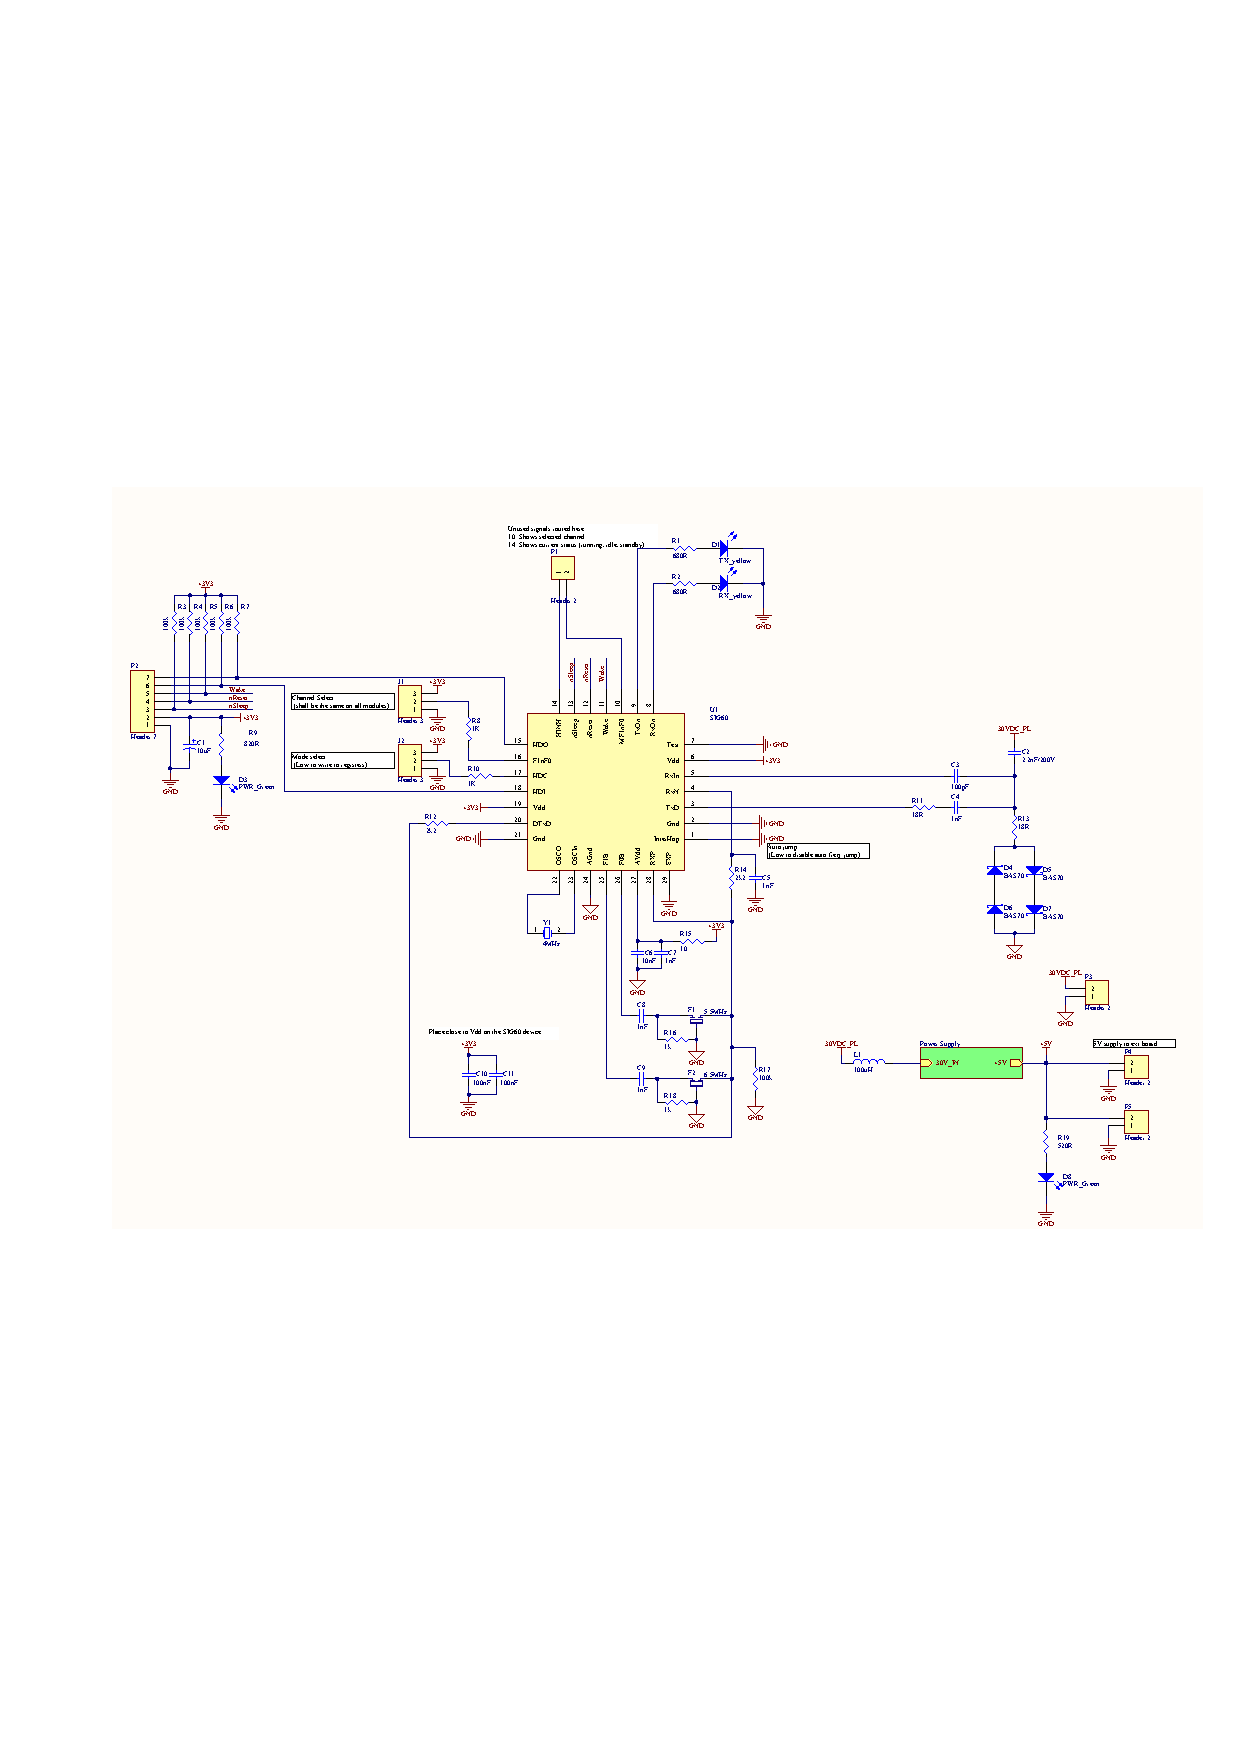
\includegraphics[width=0.9\textwidth,page=1,angle=0]{content/appendix/eudp/images/SIG60_v0_2}
		\caption{Power line circuit version 0.2}
	\end{centering}
\end{figure}

\begin{figure}[H]
	\begin{centering}
		 \includegraphics[width=0.8\textwidth,page=2,angle=0]{content/appendix/eudp/images/SIG60_v0_2}
		\caption{Power supply. 2 x 5 volt 3 ampere version 0.2.}
	\end{centering}
\end{figure}

\begin{figure}[H]
	\begin{centering}
		 \includegraphics[width=0.8\textwidth,page=3,angle=0]{content/appendix/eudp/images/SIG60_v0_2}
		\caption{PCB layout of the power line circuit and the 5 volt power supply version 0.2.}
	\end{centering}
\end{figure}

